\chapter{Immagini, tabelle, codice, liste}
In questo capitolo verranno spiegati tutti i comandi per inserire codice, tabelle di varie dimensioni, elenchi, immagini ecc.


\section{Liste}
Le liste possono essere sia numerate che puntate. La prima lista mostra come si scrivono alcuni caratteri e come si definisce lo stile di scrittura:
\begin{itemize}
    \item si può scrivere in \textbf{grassetto};
    \item si può scrivere in \textit{corsivo};
    \item si può inserire il carattere \& per la e commerciale;
    \item si può inserire il carattere \_ per l'underscore;
\end{itemize}

Ci sono anche gli elenchi numerati classici:
\begin{enumerate}
    \item primo elemento;
    \item secondo elemento;
    \item terzo elemento.
\end{enumerate}

Ma anche gli elenchi in numeri romani:
\begin{enumerate}[I]    % sostituendo 'I' con 'i' l'elenco sarà con i numeri romani minuscoli.
    \item primo elemento in romano;
    \item secondo elemento in romano;
    \item terzo elemento in romano;
    \item quarto elemento in romano.
\end{enumerate}


\section{Immagini}
Durante la produzione del testo può essere utile avere un'immagine o una serie di immagini.

\begin{figure}[H]
	\centering
	
\includegraphics[scale=0.4]{image1} % Non è necessario specificare l'estensione. L'immagine viene pescata automaticamente dalla cartella 'img' per cui non è necessario scrivere il percorso completo
	\caption{Immagine singola centrata e scalata}
	\label{capitolo2:image1}
\end{figure}

È possibile fare riferimento alle immagini attraverso la sua label (figura \ref{capitolo2:image1}).\\   % Con questo \\ si va a capo
In altri casi è necessario avere più immagini affiancate.

\begin{figure}[H]
    \centering
    \subfloat[Immagine 1]{
\includegraphics[scale=0.2]{image2a}}
    \hfill
    \subfloat[Immagine 2]{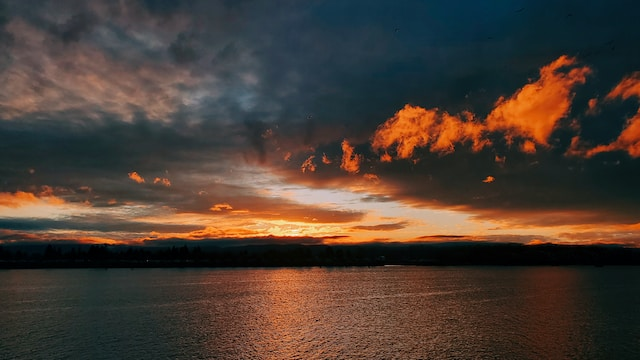
\includegraphics[scale=0.2]{image2b}}
    \hfill
    \subfloat[Immagine 3]{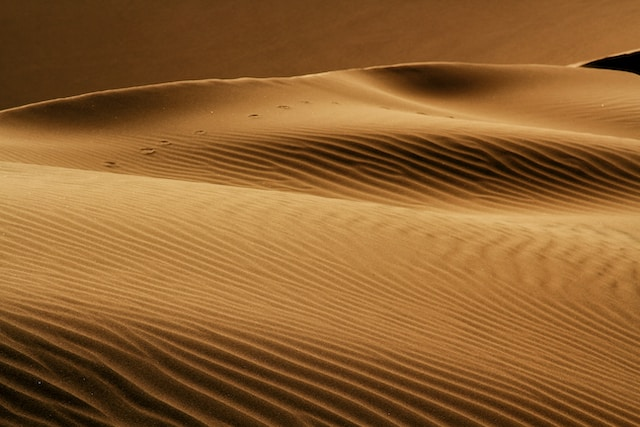
\includegraphics[scale=0.2]{image2c}}
    \hfill
    \caption{Immagini affiancate al centro}
    \label{capitolo2:immaginiAffiancate}
\end{figure}


\section{Tabelle}
Le tabelle possono avere varie dimensioni. Qui ne verranno mostrate 2: una con una dimensione normale e una con una dimensione maggiore per mostrare come si adattano alla pagina.
\begin{table}[h!]
    \centering
    \begin{tabular}{|c|c|c|}
        \hline
        \textbf{Colonna 1} & \textbf{Colonna 2} & \textbf{Colonna 3} \\
        \hline
        Dato 1 & 10 & Testo A \\
        \hline
        Dato 2 & 5.6 & Testo B \\
        \hline
        Dato 3 & 7.2 & Testo C \\
        \hline
    \end{tabular}
    \caption{Tabella piccola}
	\label{capitolo2:tabellaPiccola}
\end{table}

Quella che segue è una tabella più grande e adattata alla pagina, in modo da essere stampabile.

\begin{table}[h!]
	\centering
    \small
	\begin{tabular}{| c | c | c | c | c | c | c || c |}
		\hline \textbf{Colonna 1} & \textbf{Colonna 2} & \textbf{Colonna 3} & \textbf{Colonna 4} & \textbf{Colonna 5} & \textbf{Colonna 6} & \textbf{Colonna 7} & \textbf{Colonna 8} \\ [0.5ex]
		\hline\hline
		Dato 1 & 12 & \makecell{Testo che per \\ questioni di \\ spazio va a capo} & 3.4 & 5 & Testo X & 0.7 & \textbf{34.1} \\
		\hline
		Dato 2 & 8.9 & Testo B & 1.2 & 2 & Testo Y & 0.3 & \textbf{12.4} \\
		\hline
		Dato 3 & 15 & Testo C & 4.8 & 3 & Testo Z & 0.9 & \textbf{23.7} \\
		\hline
        Dato 4 & 6.5 & Testo D & 2.1 & 1 & Testo W & 0.5 & \textbf{10.6} \\
        \hline
        Dato 5 & 9.2 & Testo E & 5.3 & 4 & Testo V & 0.8 & \textbf{30.5} \\
        \hline
        Dato 6 & 14 & Testo F & 3.2 & 2 & Testo U & 0.4 & \textbf{21.6} \\
        \hline
        Dato 7 & 7.8 & Testo G & 1.5 & 3 & Testo T & 0.6 & \textbf{13.9} \\
        \hline
        Dato 8 & 10.1 & Testo H & 4.5 & 4 & Testo S & 0.7 & \textbf{30.3} \\
        \hline
        Dato 9 & 5.3 & Testo I & 2.8 & 1 & Testo R & 0.2 & \textbf{9.1} \\
        \hline
        Dato 10 & 11.5 & Testo J & 3.7 & 2 & Testo Q & 0.9 & \textbf{32.8} \\
        \hline
	\end{tabular}
	\caption{Tabella grande}
	\label{capitolo2:tabellaGrande}
\end{table}


\section{Codice}
Qui verranno mostrati due esempi di codice sia in Python che in JSON.

\begin{lstlisting}[language=json, basicstyle=\small, caption={Esempio JSON}, label=capitolo2:code:json]
{
  "nome": "John Doe",
  "eta": 30,
  "professione": "Ingegnere",
  "indirizzo": {"via": "Via delle Rose, 123", "citta": "Città del Sole", "cap": "12345"},
  "interessi": ["musica", "viaggi", "sport"],
  "esperienze_lavorative": [{"azienda": "ABC Inc.", "posizione": "Sviluppatore software", "periodo": "2010-2015"}, {"azienda": "XYZ Corp.", "posizione": "Project Manager", "periodo": "2015-2020"}],
  "lingue": {"inglese": "fluente", "italiano": "madrelingua", "spagnolo": "intermedio"},
  "referenze": null,
  "disponibile": true
}
\end{lstlisting}

Ecco un esempio del linguaggio Python.

\begin{lstlisting}[language=python, basicstyle=\small, caption={Esempio Python}, label=capitolo2:code:python]
def somma(a, b):
return a + b

numero1 = 5
numero2 = 7

risultato = somma(numero1, numero2)
print("La somma di", numero1, "e", numero2, "è:", risultato)

\end{lstlisting}


\section{Formule matematiche}
È possibile inserire formule matematiche durante il testo e ce ne sono di due tipi. La prima si inserisce all'interno del testo: $f(x) = \frac{x^2}{2}$, mentre il secondo si inserisce in una nuova riga.
\begin{equation}
    \sum_{i=0}^{\infty} \alpha\sin{x_i}
    \label{capitolo2:eq:esempioEquazione}
\end{equation}
Anche in questo caso, tramite la label, è possibile fare riferimento a questa formula in qualsiasi punto del documento, esattamente come per immagini, tabelle e codice.